\documentclass{article}
\usepackage[utf8]{inputenc}
\usepackage{amsmath}
\usepackage{amssymb}
\usepackage{amsthm}
\usepackage{enumerate}
\usepackage{mathtools}
\usepackage{float} % For plassering av bilder
\usepackage{a4wide} % mer width
\usepackage{amsmath}
\usepackage{amssymb}
\usepackage{parskip}
\usepackage{xcolor} % Fargelegger matriseelement
\usepackage{verbatim}
\usepackage{makecell} % formatere celler i tabell
\usepackage{subfig}


\usepackage[colorlinks=false,allcolors=blue]{hyperref}
%Fikser hyperref
\addto\extrasnorsk{%
\def\figureautorefname{Figure}%
\def\tableautorefname{Table}%
\def\sectionautorefname{section}%
\def\subsectionautorefname{subsection}%
}
% Vi endrer fonten som brukes for URLer til den vanlige tekstfonten.
\urlstyle{same}


%Tikz
\usepackage[american]{circuitikz}
\usepackage{tikz}
\usetikzlibrary{patterns}
\usetikzlibrary{arrows.meta}
\usepackage{pgfplots}

% FRA IC
\usepackage{natbib}
\usepackage{amsmath}
\usepackage{listings}
\usepackage{graphicx}

\usepackage[inline]{enumitem}
 \usepackage{booktabs}
\date{}
\newcommand*{\boxednumber}[1]{%
    \expandafter\readdigit\the\numexpr#1\relax\relax
}
\newcommand*{\readdigit}[1]{%
    \ifx\relax#1\else
        \boxeddigit{#1}%
        \expandafter\readdigit
    \fi
}
% Format macro used for every digit, adjust to your liking:
\newcommand*{\boxeddigit}[1]{\fbox{#1}\hspace{-\fboxrule}}

\usepackage[left=4cm,right=4cm,vmargin=1.5cm,footnotesep=0.5cm]{geometry}
\setlength\parindent{0pt}


\title{TDT4265 - Computer Vision and Deep Learning \\Assignment 4}
\author{Jakob Vahlin & Kristian Stensgård}
%\date{September 2020}

\begin{document}

\maketitle

\tableofcontents
\newpage

\section{Task 1: Object Detection Metrics}
\subsection{Task a: Intersection over union}
The intersection over union is a measurement of the overlap between two boundaries. This is used to determine how much of the predicted boundary overlaps with the actual boundary. The measurement is defined as the ratio between the area of the intersection between the two boundaries, and the area of the union over the two boundaries. An illustration of intersection of union is given in \autoref{fig:iou}

\begin{equation}
    \text{IoU} = \frac{\text{Intersection}}{\text{Union}}
\end{equation}

\begin{figure}[H]
    \centering
    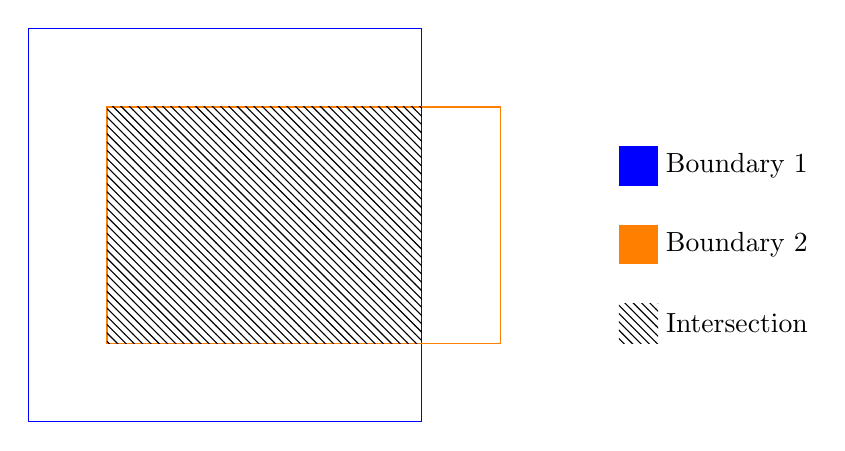
\begin{tikzpicture}
    \draw[blue] (0,0) rectangle (5,5);
    \draw[orange] (1,1) rectangle (6,4);
    \fill [pattern=north west lines] (1,1) rectangle (5,4);
    
    \fill[blue] (7.5,3) rectangle (8,3.5);
    \node at (9,3.25) {Boundary 1};
    
    \fill[orange] (7.5,2) rectangle (8,2.5);
    \node at (9,2.25) {Boundary 2};
    
    \fill[pattern=north west lines] (7.5,1) rectangle (8,1.5);
    \node at (9,1.25) {Intersection};
    %\draw [pattern=north west lines] (7.5,1) rectangle (8,1.5);
    
    \end{tikzpicture}
    \caption{An illustration of intersection over union.}

    \label{fig:iou}
\end{figure}


\subsection{Task b: Precision \& Recall}
A \textit{true positive} is a prediction that was predicted as positive, and was correct. A \textit{false positive} is a prediction that was predicted as positive, but was not correct.

Precision is a measurement of the accuracy of the predictions. It measures to what extent the predictions were correct. It is defined as the fraction between the true positives and the sum of the true and false positives, defined in \autoref{eq:precision}.

\begin{equation}
    \text{Precision} = \frac{\text{Number of True Positives}}{\text{Number of True Positives} + \text{Number of False Positives}}
    \label{eq:precision}
\end{equation}

Recall is a measurement of the extent the model is able to determine the positives. It is defined as the ratio between the True Positive predictions and the sum of the True Positive predictions and False negative predictions, where a \textit{false negative} is a negative prediction that was wrong. Mathematically, recall is defined in \autoref{eq:recall}.

\begin{equation}
    \text{Recall} = \frac{\text{Number of True Positives}}{\text{Number of True Positives} + \text{Number of false positives}}
    \label{eq:recall}
\end{equation}

\subsection{Task c:}
Given the precision and recall curves defined in \autoref{eq:curve_1} and \autoref{eq:curve_2}, the mean average precision (mAP) is defined as the mean of the average precision for each of the curves. Thus, the first step is to calculate the average precision (AP) for each of the precision and recall curves.
\begin{equation}
    P_1 = [1.0, 1.0, 1.0, 0.5, 0.2], \quad R_1 = [0.05, 0.1, 0.4, 0.7, 1.0]
    \label{eq:curve_1}
\end{equation}
\begin{equation}
    P_2 = [1.0, 0.8, 0.6, 0.5, 0.2], \quad R_2 = [0.3, 0.4, 0.5, 0.7, 1.0]
    \label{eq:curve_2}
\end{equation}

To calculate the AP for each of the curves, interpolation is used to fit the precision values on the recall interval $R_{1,2}_{\text{interpol}} = [0.0, 0.1, \dots, 1.0]$. For a given recall, $r_i$, the precision value is replaced with the maximum precision value for any recall $r \geq r_i$. The interpolated precision values with the corresponding recall interval, are given in \autoref{eq:interpol_1} and \eqref{eq:interpol_2} for curves 1 and 2 respectively.

\begin{align}
\begin{split}
    P_1_{\text{interpol}} &= [1.0, 1.0, 1.0, 1.0, 1.0, 0.5, 0.5,0.5, 0.2, 0.2, 0.2] \\
    R_1_{\text{interpol}} &= [0.0, 0.1, 0.2, 0.3, 0.4, 0.5, 0.6, 0.7, 0.8, 0.9, 1.0]
\end{split}
\label{eq:interpol_1}
\end{align}
\begin{align}
\begin{split}
    P_2_{\text{interpol}} &= [1.0, 1.0, 1.0, 1.0, 0.8, 0.6, 0.5, 0.5, 0.2, 0.2, 0.2] \\ 
    R_2_{\text{interpol}} &= [0.0, 0.1, 0.2, 0.3, 0.4, 0.5, 0.6, 0.7, 0.8, 0.9, 1.0]
\end{split}
\label{eq:interpol_2}
\end{align}

Thus the AP for the respective curves is found by computing the average of both sets of precision values.

\begin{align}
\begin{split}
AP_1 &= \frac{1}{11} \sum_{i = 1}^{11}  P_1_i \\
    &= \frac{(5\cdot 1) + (3\cdot 0.5) + (3\cdot 0.2)}{11}\\
    &= 0.645
\end{split}
\label{eq:ap_1}
\end{align}
\begin{align}
\begin{split}
AP_2 &= \frac{1}{11} \sum_{i = 1}^{11}  P_2_i \\
    &= \frac{(4\cdot 1) + (1\cdot 0.8) + (1\cdot 0.6) + (2\cdot 0.5) + (3\cdot 0.2)}{11}\\
    &= 0.636
\end{split}
\label{eq:ap_2}
\end{align}

Finally, the mean average precision is found by computing the average of the two values found in \autoref{eq:ap_1} and \autoref{eq:ap_2}. 

\begin{equation}
    \text{mAP} = \frac{0.636 + 0.645}{2} = 0.641
\end{equation}

\section{Task 2: Implementing Mean Average Precision}
\subsection{Task f}
When running the task2.py script the mean average precision was $0.9835$.
The precision-recall curve for this task is plotted in \autoref{fig:prc}.
\begin{figure}[H]
    \centering
    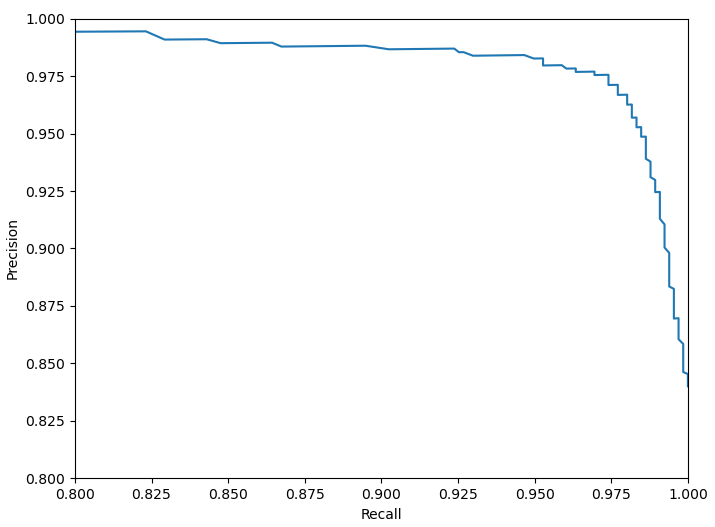
\includegraphics[width=\textwidth]{Assignments/Assignment_4/plots/precision_recall_curve.png}
    \caption{Precision-recall curve for task 2}
    \label{fig:prc}
\end{figure}

\section{Task 3: Theory}

\subsection{Task a}
%  The SSD architecture produces a fixed-size number of bounding boxes and a score for each
% bounding box. When performing inference with SSD, we need to filter out a set of overlapping
% boxes. What is this filtering operation called?
 

SSD uses non-maximum suppression to remove overlapping boxes. If these boxes were not removed, then SSD would have duplicate predictions pointing to the same object.

\subsection{Task b}
% The SSD architecture predicts bounding boxes at multiple scales to enable the network to
% detect objects of different sizes.
% Is the following true or false: Predictions from the deeper layers in SSD are responsible to
% detect small object
\textbf{False}

The feature maps with highest resolution are responsible for detecting small object. Conversely the lower resolution feature maps are used for detecting large objects. The high resolution feature maps are at the top/beginning of the network and this is where detection of small objects are done. The deep layers towards the end of the network are responsible for detection of the large objects.

\subsection{Task c}

% SSD use k number of ”anchors” 2 with different aspect ratios at each spatial location in a
% feature map to predict c class scores and 4 offsets relative to the original box shape.
% Why do they use different bounding box aspect ratios at the same spatial location?

If the bounding box aspect ratios were all the same, then the model will become good at predicting one category corresponding to a default box with that shape. However, predictions for objects with others shapes corresponding to other box aspect ratios would be poor. This will make initial training poor. 

By using different aspect ratios one can improve training and the models ability to detect object of different sizes.



\subsection{Task d}
% What is the main difference between SSD and YOLOv1/v2 (The YOLO version they refer
% to in the SSD paper)?

The SSD model adds several feature layers to the end of a base network, which predict the offsets to default boxes of different scales and aspect ratios and their associated confidences. The YOLO model uses a CNN feature extractor, much like the SSD model. The YOLO however does regression using two convolutional layers at the end to make boundary box predictions. 

% A:
% Compared to YOLO, SSD is significantly more accurate,
% likely due to the use of convolutional default boxes from multiple feature maps and our
% matching strategy during training.
% A key feature of our model is the use of multi-scale convolutional bounding box outputs
% attached to multiple feature maps at the top of the network. This representation allows
% us to efficiently model the space of possible box shapes.


\subsection{Task e}
% Given a SSD framework, where the first scale the network predicts at is at the last feature
% map with a resolution of 38 × 38 (H × W). For each anchor location, we place 6 different anchors
% with different aspect ratios. How many anchors boxes do we have in total for this feature map?

Given a feature map with spatial dimensions $38 \times 38$ and 6 anchors with different aspect ratios at each anchor location we get:

\begin{equation}
    38 \cdot 38 \cdot 6 = 8,664
\end{equation}
So in total we 8,664 anchor boxes for this feature map.



\subsection{Task f}
% The network outlined in the previous subtask predicts at multiple resolutions, specifically
% 38 × 38, 19 × 19, 10 × 10, 5 × 5, 3 × 3 and 1 × 1. It uses 6 different aspect ratios at each location in
% every feature map as anchors. How many anchors boxes do we have in total for the entire network?
Considering a newtwork that predicts at the resolutions $38 \times 38$, $19 \times 19$, $10 \time 10$, $5 \times 5$, $3 \times 3$ and $1 \times 1$ with 6 different aspect ratios at every anchor point, the total number of anchor boxes is:

\begin{equation}
    6\cdot(38^2 + 19^2 + 10^2 + 5^2 + 3^2 + 1^2) = 11,640
\end{equation}


\section{Task 4: Implementing Single Shot Detector}


\subsection{Task b}
The network mentioned outlined in \autoref{tab:base_net} was implemented as the backbone for the SSD described in the assignment description.Each convolutional layer has a kernel size of 3 × 3 and padding of 1. Each MaxPool2D layer has a kernel size of 2 × 2. The goal was to achieve a mAP value in the range $[75\%,77\%]$ within 6 000 iterations. The goal was accomplished, with the model reaching a mAP of \textbf{75.7}\% after 6 000 iterations. 

The total loss and mAP is plotted against the training iterations in \autoref{fig:loss4b} and \autoref{fig:mAP4b} respectively.

\begin{figure}[H]
    \centering
    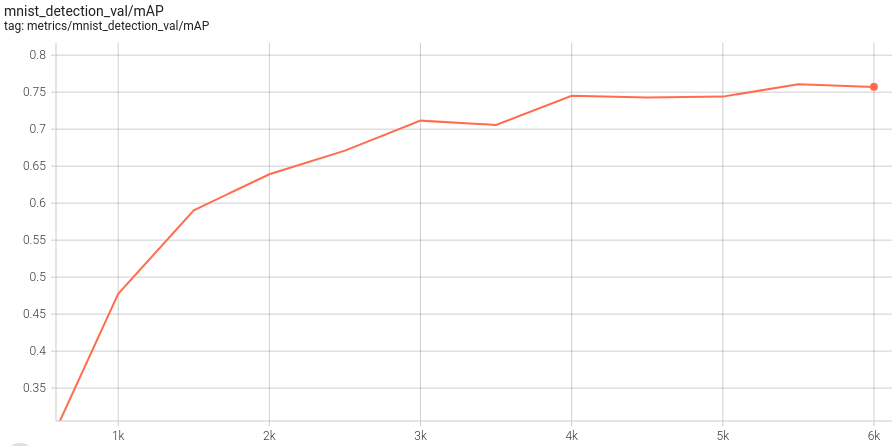
\includegraphics[width=\textwidth]{Assignments/Assignment_4/plots/map_nonsmooth.png}
    \caption{mAP for the SSD using the backbone outlined in ...}
    \label{fig:mAP4b}
\end{figure}


\begin{figure}[H]
    \centering
    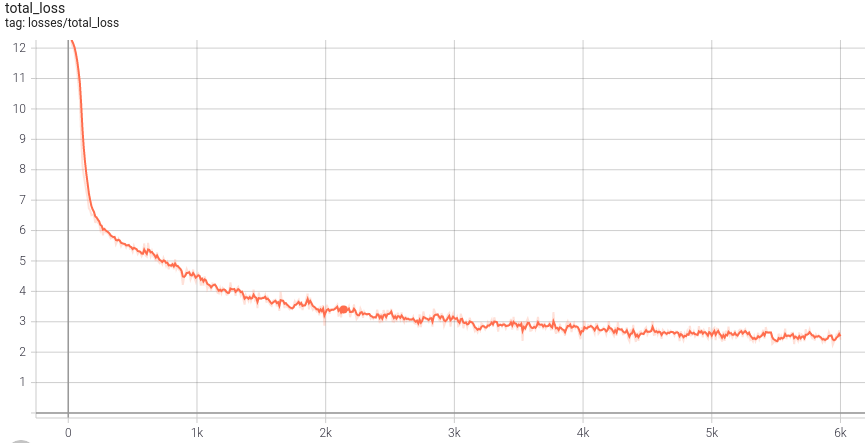
\includegraphics[width=\textwidth]{Assignments/Assignment_4/plots/tot_loss_full.png}
    \caption{Total loss for the SSD using the backbone outlined in ...}
    \label{fig:loss4b}
\end{figure}


\begin{table}[H]
\caption{The network used as the backbone for the SSD in task 4b. Each convolutional layer has a kernel size of $3 \times 3$ and padding of
1. Each MaxPool2D layer has a kernel size of $2 \times 2$. \textbf{*}\textit{The last
convolution have a stride of 1, padding of 0, and a kernel size of 3 × 3}
}
\label{tab:base_net}
\begin{tabular}{l|c|c|c}
\hline
Is Output & \multicolumn{1}{l|}{Layer Type} & \multicolumn{1}{l|}{Number of Filters} & \multicolumn{1}{l}{Stride} \\ \hline
 & Conv2D & 32 & 1 \\
 & MaxPool2D & - & 2 \\
 & ReLU & - & - \\
 & Conv2D & 64 & 1 \\
 & MaxPool2D & - & 2 \\
 & ReLU & - & - \\
 & Conv2D & 64 & 1 \\
 & ReLU & - & - \\
Yes - Resolution: 38 × 38 & Conv2D & 128 & 2 \\ \hline
 & ReLU & - & - \\
 & Conv2D & 128 & 1 \\
 & ReLU & - & - \\
Yes - Resolution: 19 × 19 & Conv2D & 256 & 2 \\ \hline
 & ReLU & - & - \\
 & Conv2D & 256 & 1 \\
 & ReLU & - & - \\
Yes - Resolution: 9 × 9 & Conv2D & 128 & 2 \\ \hline
 & ReLU & - & - \\
 & Conv2D & 128 & 1 \\
 & ReLU & - & - \\
Yes - Resolution: 5 × 5 & Conv2D & 128 & 2 \\ \hline
 & ReLU & - & - \\
 & Conv2D & 128 & 1 \\
 & ReLU & - & - \\
Yes - Resolution: 3 × 3 & Conv2D & 64 & 2 \\ \hline
 & ReLU & - & - \\
 & Conv2D & 128 & 1 \\
 & ReLU & - & - \\
Yes - Resolution: 1 × 1 * & Conv2D & 64 & 1 \\ \hline
\end{tabular}
\end{table}


\subsection{Task c}
In order to increase the mean average precision of the detector from task 4b to reach a mAP value of $85\%$ within 10 000 iterations, modifications and additions to the model have been implemented. 

Based on experience from Assignment 3, the first attempt at increasing the mAP involved adding more data augmentation, as this was the modification that resulted in the biggest performance boost in Assignment 3. However, augmenting the dataset by adding flipping and rotation to the training set resulted in poor performance. Thus no data augmentation was used in the final successful model. 

The number of filters in the convolutional network was extended, motivated by the success when extending the layers from Assignment 3. More specifically, the number of filters in the third convolutional layer was extended from 128 to 256. This change increased the performance.

Furthermore, reducing the learning rate from $2\cdot 10^{-3}$ to $1.2\cdot 10^{-3}$ as well as adding batch normalization at certain layers also slighly improved the performance.   


The final network architecture of the improved network is outlined in \autoref{tab:modified_net_4c}.

The final change to the SSD, that also yielded the biggest performance leap, was altering the sizes of the default boxes. This was done after it was discovered that the detector performed poorly on smaller objects. In an effort to improved the detection on smaller objects, the minimum and maximum dimensions of the first default box was changed from $[30,30]$ to $[15,15]$ and $[60,60]$ to $[30,30]$ respectively. 

With these changes the model reached a mean average precision of \textbf{87.93}\% after 10 000 iterations, exceeding the desired target value of $85\%$. The desired target value of 85\% was exceed after 5000 gradient descent iterations, with a mean average precision of 85.7\%. 
Plots showing the mean average precision and total loss are shown in \autoref{fig:4c_map} and \autoref{fig:4c_loss} respectively.

\begin{figure}[H]
    \centering
    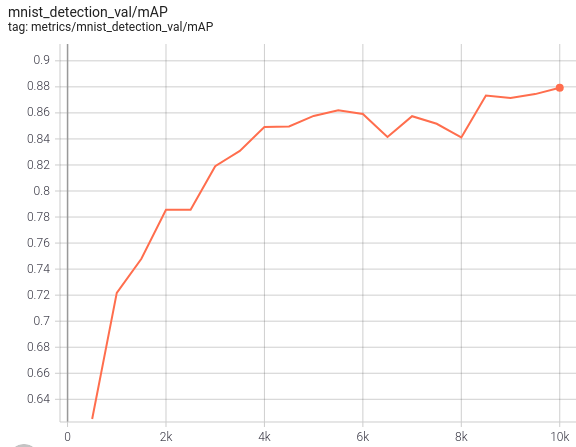
\includegraphics[width=\textwidth]{Assignments/Assignment_4/plots/map_medium.png}
    \caption{The development of mean average precision values during training. }
    \label{fig:4c_map}
\end{figure}


\begin{figure}[H]
    \centering
    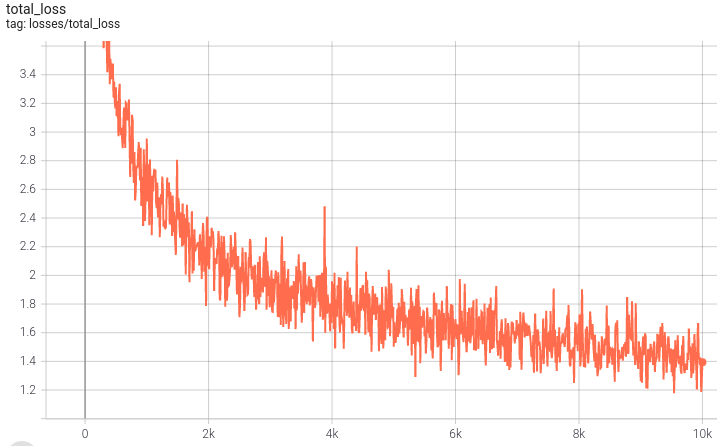
\includegraphics[width=\textwidth]{Assignments/Assignment_4/plots/tot_loss_medium.png}
    \caption{The development of the training loss values during training.}
    \label{fig:4c_loss}
\end{figure}


\begin{table}[H]
\caption{The modified network used as the backbone for the SSD in task 4c. Each convolutional layer has a kernel size of $3 \times 3$ and padding of 1. Each MaxPool2D layer has a kernel size of $2 \times 2$. \textbf{*}\textit{The last
convolution should have a stride of 1 and padding of 0}
}
\label{tab:modified_net_4c}
\begin{tabular}{l|c|c|c}
\hline
Is Output & \multicolumn{1}{l|}{Layer Type} & \multicolumn{1}{l|}{Number of Filters} & \multicolumn{1}{l}{Stride} \\ \hline
 & Conv2D & 32 & 1 \\
 & MaxPool2D & - & 2 \\
 & ReLU & - & - \\
 & Conv2D & 64 & 1 \\
 & MaxPool2D & - & 2 \\
 & ReLU & - & - \\
 & Conv2D & 128 & 1 \\
   & BatchNorm2D & - & - \\
 & ReLU & - & - \\
Yes - Resolution: 38 × 38 & Conv2D & 128 & 2 \\ \hline
 & ReLU & - & - \\
 & Conv2D & 128 & 1 \\
 & ReLU & - & - \\
    & BatchNorm2D & - & - \\
Yes - Resolution: 19 × 19 & Conv2D & 256 & 2 \\ \hline
 & ReLU & - & - \\
 & Conv2D & 256 & 1 \\
 & ReLU & - & - \\
    & BatchNorm2D & - & - \\
Yes - Resolution: 9 × 9 & Conv2D & 256 & 2 \\ \hline
 & ReLU & - & - \\
 & Conv2D & 256 & 1 \\
 & ReLU & - & - \\
    & BatchNorm2D & - & - \\
Yes - Resolution: 5 × 5 & Conv2D & 256 & 2 \\ \hline
 & ReLU & - & - \\
 & Conv2D & 128 & 1 \\
 & ReLU & - & - \\
    & BatchNorm2D & - & - \\
Yes - Resolution: 3 × 3 & Conv2D & 64 & 2 \\ \hline
 & ReLU & - & - \\
 & Conv2D & 128 & 1 \\
 & ReLU & - & - \\
    & BatchNorm2D & - & - \\
Yes - Resolution: 1 × 1 * & Conv2D & 64 & 1 \\ \hline
\end{tabular}
\end{table}


\subsection{Task d}

Having reached a mAP of 87.93\% the model was further improved in an effort to reach a mean average precision of $90\%$ or greater within 15 000 timesteps. 

It was found that the only modification needed to surpass the target value was to further adjust the minimum and maximum values of the default boxes, as discussed in task 4c. Instead of just changing the first default box, the first 3 default boxes was modified. The changes to first 3 default boxes are shown in \autoref{tab:boundary_boxes_4d}. The rest of the network is identical to the one described in task 4c. The network reached 90.2\% mAP on the validation set after training was done.




Plots showing the mean average precision and total loss are shown in \autoref{fig:4dmap} and \autoref{fig:4dloss} respectively. 
\begin{table}[H]
\centering
\caption{Original and modified minimum and maximum sizes of the first 3 default boxes in the SSD. The other 3 default boxes have not been modified and are left out.}
\label{tab:boundary_boxes_4d}
\begin{tabular}{|l|l|l|}
\hline
\textbf{Box} & \textbf{Original size}                                                    & \textbf{Modified size}                                                  \\ \hline
1            & \begin{tabular}[c]{@{}l@{}}MIN:  [30,30] \\ MAX:[60,60]\end{tabular}      & \begin{tabular}[c]{@{}l@{}}MIN:  [15,15]\\ MAX:[30,30]\end{tabular}     \\ \hline
2            & \begin{tabular}[c]{@{}l@{}}MIN:   [60,60]\\ MAX: [111,111]\end{tabular}   & \begin{tabular}[c]{@{}l@{}}MIN:   [30,30]\\ MAX: [50,50]\end{tabular}   \\ \hline
3            & \begin{tabular}[c]{@{}l@{}}MIN:   [111,111]\\ MAX: [162,162]\end{tabular} & \begin{tabular}[c]{@{}l@{}}MIN:   [80,80]\\ MAX: [130,130]\end{tabular} \\ \hline
\end{tabular}
\end{table}

\begin{figure}[H]
    \centering
    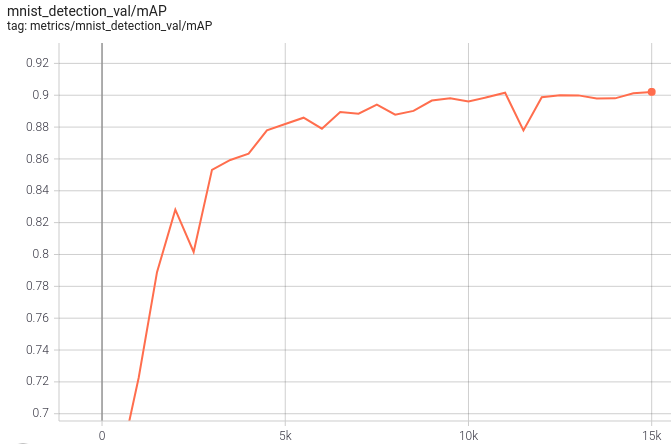
\includegraphics[width=\textwidth]{Assignments/Assignment_4/plots/mAp_hard.png}
    \caption{The development of mean average precision values during training for the improved model.}
    \label{fig:4dmap}
\end{figure}

\begin{figure}[H]
    \centering
    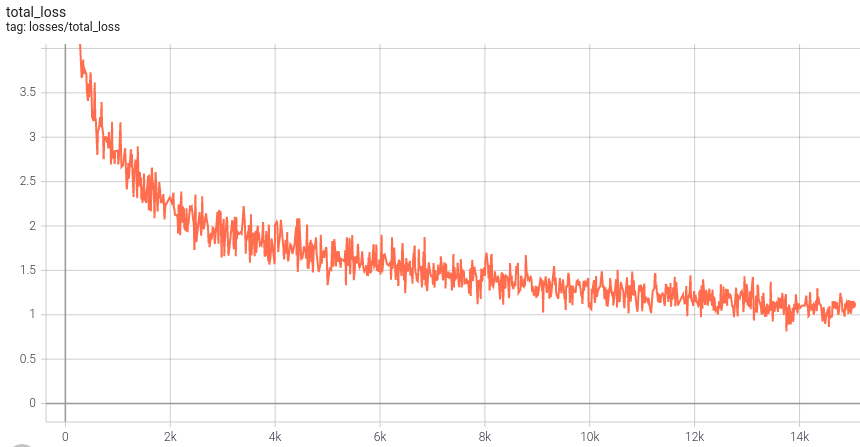
\includegraphics[width=\textwidth]{Assignments/Assignment_4/plots/tot_loss_hard.png}
    \caption{The development of total loss values during training for the improved model.}
    \label{fig:4dloss}
\end{figure}




\subsection{Task e}
The trained model from the previous task that reached 90.2\% mAP was tested on 15 of the images from the yymnist validation set. The score threshold used for this test was 0.7. The resulting prediction boxes and their category was placed on top of these images.
The results are shown in \autoref{fig:test1} to \autoref{fig:test7}. In these images we see that the detector performs quite well, but struggles a bit with numbers that are very close to each other, like in the right image in \autoref{fig:test5}. Some digits are quite obvious for us humans, but apparently the detector fails to detect the 7 and 6 in the right images in \autoref{fig:test3} and \autoref{fig:test4}. There are also more examples of clearly distinguishable numbers that have not been detected. Lowering the score threshold will most likely give better results.




\begin{figure}[H]%
    \centering
    {{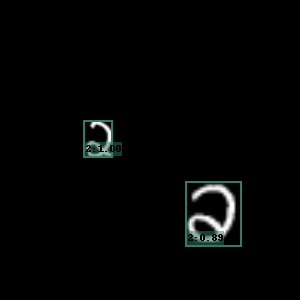
\includegraphics[width=6cm]{Assignments/Assignment_4/plots/0.png} }}%
    \qquad
    {{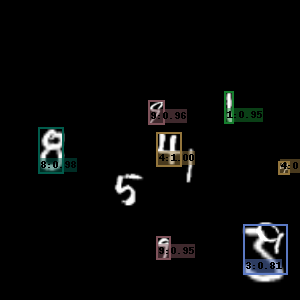
\includegraphics[width=6cm]{Assignments/Assignment_4/plots/1.png} }}%
    \caption{Two of the test images side by side}%
    \label{fig:test1}%
\end{figure}


\begin{figure}[H]%
    \centering
   {{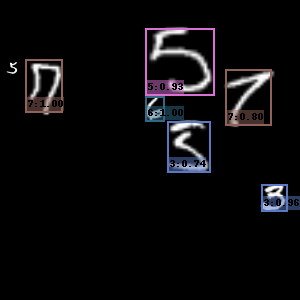
\includegraphics[width=6cm]{Assignments/Assignment_4/plots/2.png} }}%
    \qquad
    {{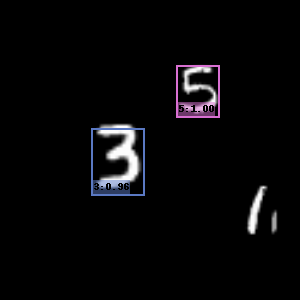
\includegraphics[width=6cm]{Assignments/Assignment_4/plots/3.png} }}%
    \caption{Two of the test images side by side}%
    \label{fig:test}%
\end{figure}

\begin{figure}[H]%
    \centering
    {{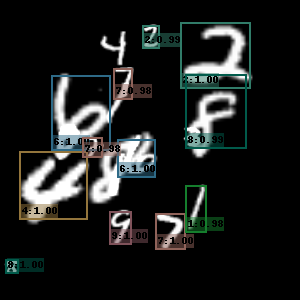
\includegraphics[width=6cm]{Assignments/Assignment_4/plots/4.png} }}%
    \qquad
    {{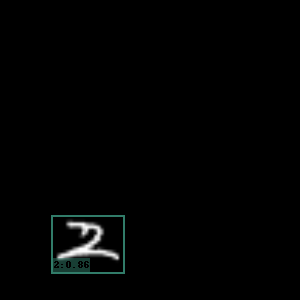
\includegraphics[width=6cm]{Assignments/Assignment_4/plots/5.png} }}%
    \caption{Two of the test images side by side}%
    \label{fig:test2}%
\end{figure}

\begin{figure}[H]%
    \centering
    {{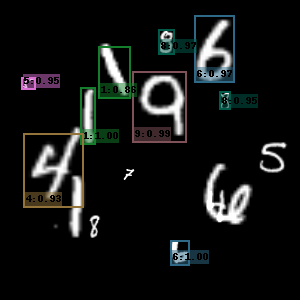
\includegraphics[width=6cm]{Assignments/Assignment_4/plots/6.png} }}%
    \qquad
   {{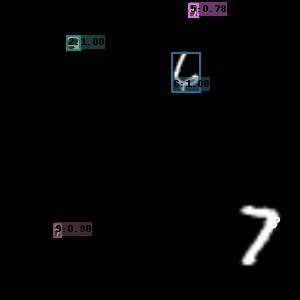
\includegraphics[width=6cm]{Assignments/Assignment_4/plots/7.png} }}%
    \caption{Two of the test images side by side}%
    \label{fig:test3}%
\end{figure}

\begin{figure}[H]%
    \centering
    {{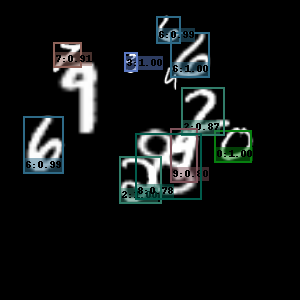
\includegraphics[width=6cm]{Assignments/Assignment_4/plots/8.png} }}%
    \qquad
    {{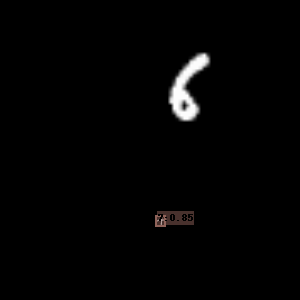
\includegraphics[width=6cm]{Assignments/Assignment_4/plots/9.png} }}%
    \caption{Two of the test images side by side}%
    \label{fig:test4}%
\end{figure}


\begin{figure}[H]%
    \centering
    {{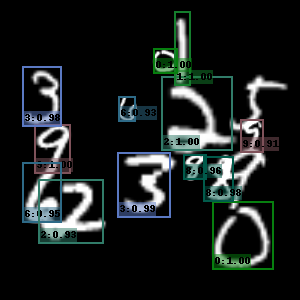
\includegraphics[width=6cm]{Assignments/Assignment_4/plots/10.png} }}%
    \qquad
    {{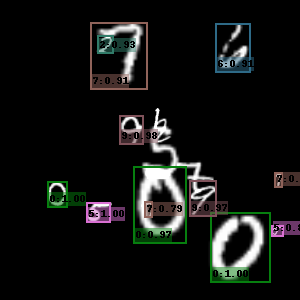
\includegraphics[width=6cm]{Assignments/Assignment_4/plots/11.png} }}%
    \caption{Two of the test images side by side}%
    \label{fig:test5}%
\end{figure}

\begin{figure}[H]%
    \centering
    {{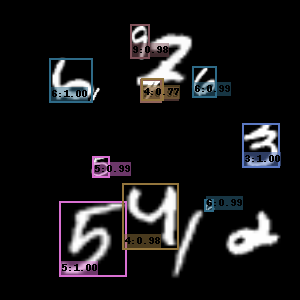
\includegraphics[width=6cm]{Assignments/Assignment_4/plots/12.png} }}%
    \qquad
    {{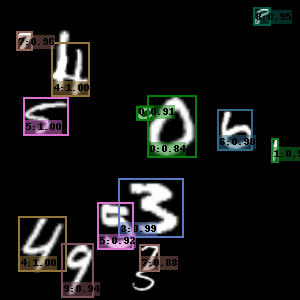
\includegraphics[width=6cm]{Assignments/Assignment_4/plots/13.png} }}%
    \caption{Two of the test images side by side}%
    \label{fig:test6}%
\end{figure}


\begin{figure}[H]
    \centering
    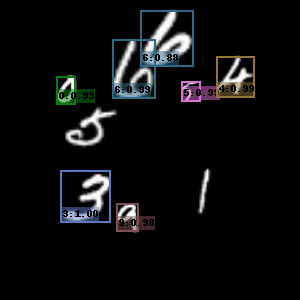
\includegraphics[width=\textwidth]{Assignments/Assignment_4/plots/14.png}
    \caption{The final test image}
    \label{fig:test7}
\end{figure}




\subsection{Task f}
For the last task a the pretrained network VGG16 was used as a backbone for the detector. The detector was trained for 5000 gradient descent iterations on the VOC dataset. The mAp and total loss is shown in \autoref{fig:vgg_map} and \autoref{fig:vgg_loss}.


The trained detector was tested on five images from the PASCAL VOC dataset and the resulting predicted boxes and their category is shown in \autoref{fig:voc1}, \autoref{fig:voc2} and \autoref{fig:voc3}. The score threshold used for this test was $0.2$.


\begin{figure}[H]
    \centering
    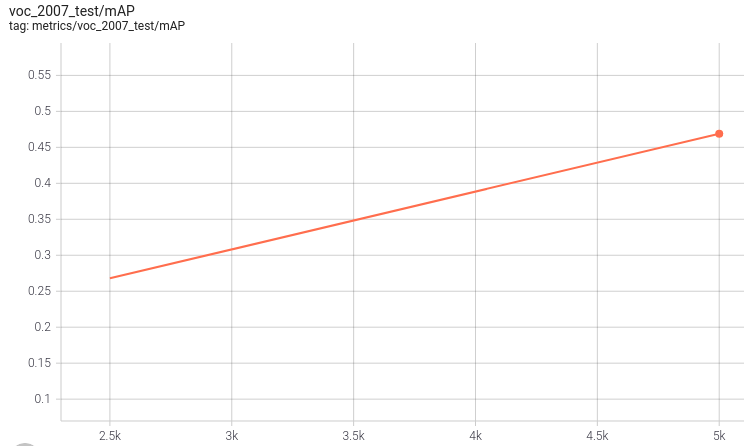
\includegraphics[width=\textwidth]{Assignments/Assignment_4/plots/vgg/map_vgg.png}
    \caption{Caption}
    \label{fig:vgg_map}
\end{figure}



\begin{figure}[H]
    \centering
    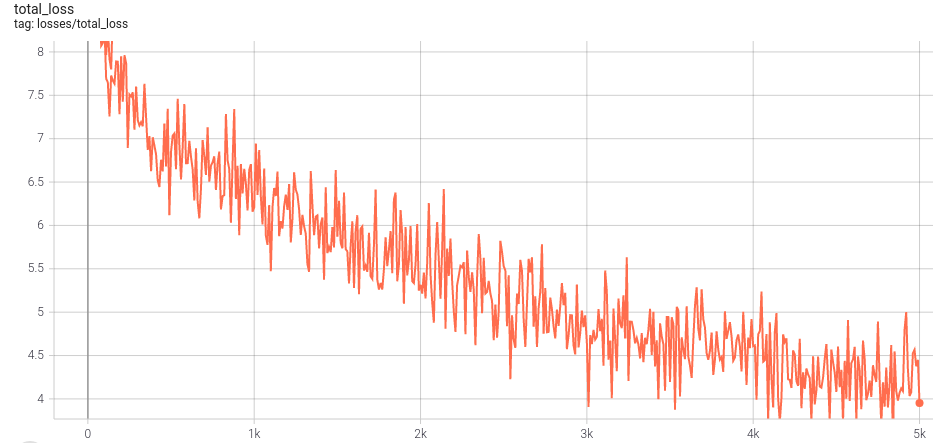
\includegraphics[width=\textwidth]{Assignments/Assignment_4/plots/vgg/tot_loss_vgg.png}
    \caption{Caption}
    \label{fig:vgg_loss}
\end{figure}



\begin{figure}[H]%
    \centering
    \subfloat[\centering TV-monitor labeled as person, and person labeled correctly]{{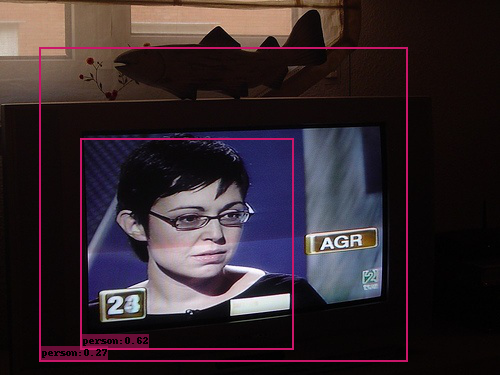
\includegraphics[width=6cm]{Assignments/Assignment_4/plots/vgg/000342.png} }}%
    \qquad
    \subfloat[\centering Cat labeled as a dog.]{{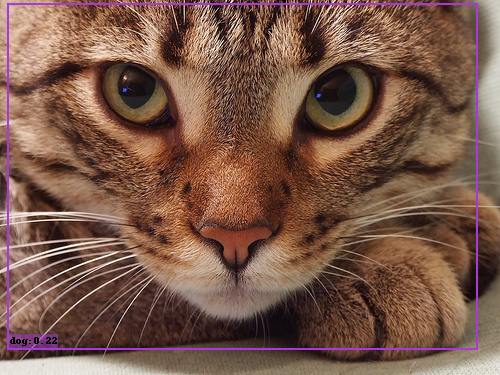
\includegraphics[width=6cm]{Assignments/Assignment_4/plots/vgg/000542.png} }}%
    \caption{Two of the test images side by side}%
    \label{fig:voc1}%
\end{figure}

\begin{figure}[H]%
    \centering
    \subfloat[\centering Image of a dinner party with a lot of accurate prediction boxes]{{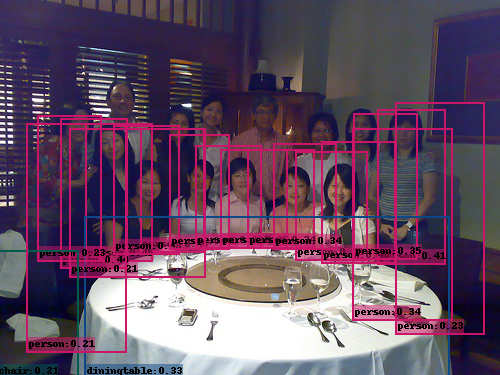
\includegraphics[width=6cm]{Assignments/Assignment_4/plots/vgg/003123.png} }}%
    \qquad
    \subfloat[\centering Person on sofa with correct labels, but very large prediction box for persoon 2]{{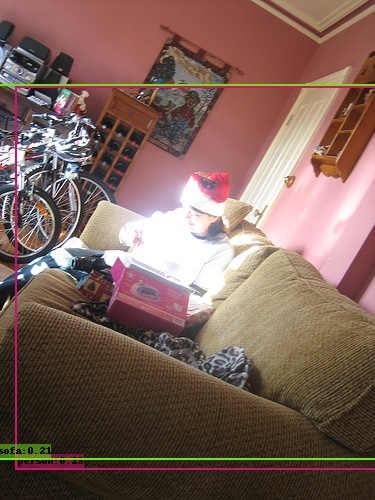
\includegraphics[width=6cm]{Assignments/Assignment_4/plots/vgg/004101.png} }}%
    \caption{Two of the test images side by side}%
    \label{fig:voc2}%
\end{figure}


\begin{figure}[H]
    \centering
    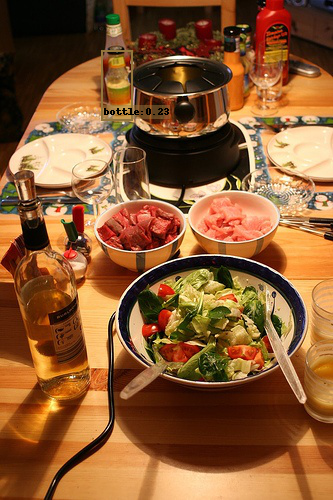
\includegraphics[width=\textwidth]{Assignments/Assignment_4/plots/vgg/008591.png}
    \caption{Dinner table with only a bottle labeled and bounded by a prediction box.}
    \label{fig:voc3}
\end{figure}

\end{document}